% !TEX root = main.tex

\subsection{上板}
\qquad 几条代表性指令的Basys3板结果如下,其他指令结果见具体实现。从左到右从上到下四幅图依次是:当前/下条PC、rs寄存器地址/值、rt寄存器地址/值、ALU结果输出/DB总线数据。\textcolor{red}{注意这里显示的都是最后一个状态的值。又由于这些信号都采用wire类型,故写入寄存器后可能导致alu\_res的相应改变。}但可以看见上板结果与前面仿真分析的结果相同,这成功证明了程序的正确性。
\begin{enumerate}
    \item 0x00: \verb'addiu $1, $0, 8'
    \begin{figure}[H]
    \centering
    \begin{tabular}{cc}
    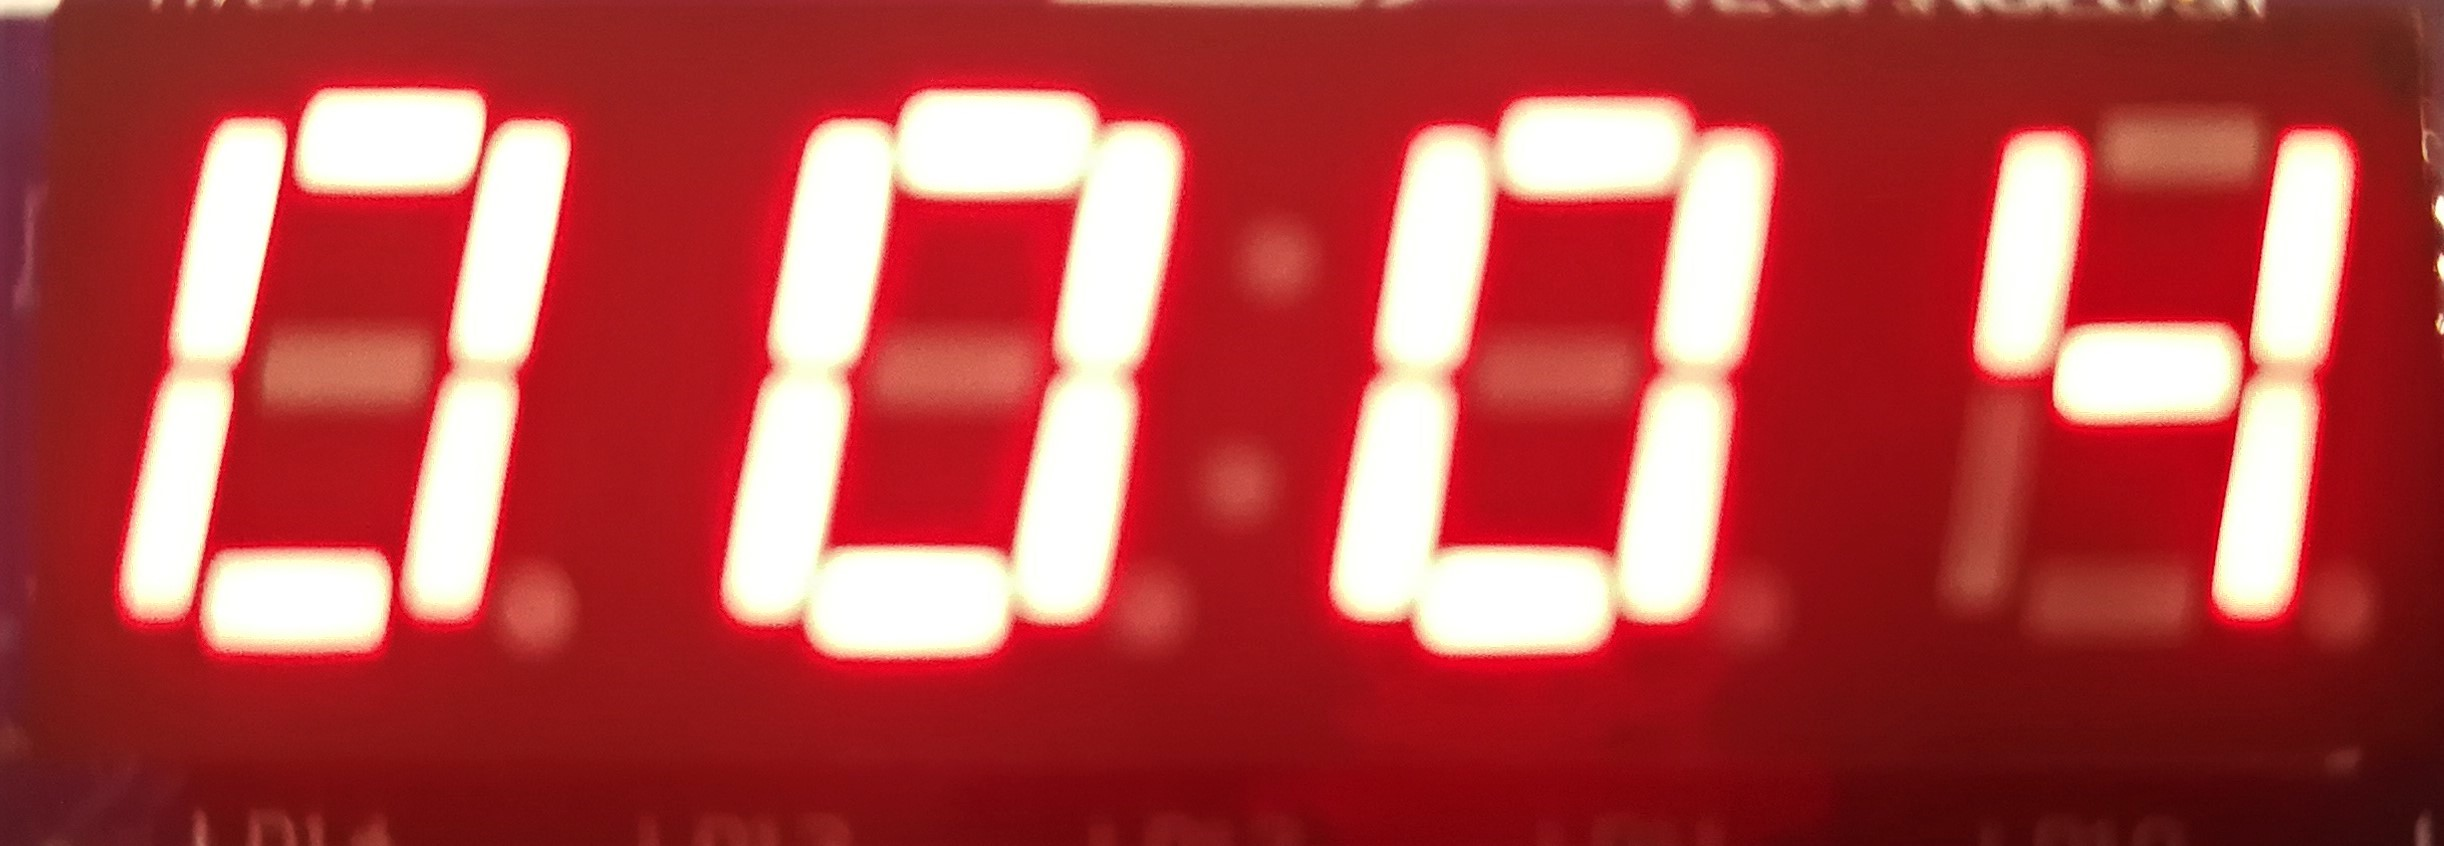
\includegraphics[width=0.3\linewidth]{fig/Implementation/0x00_00.jpg}&
    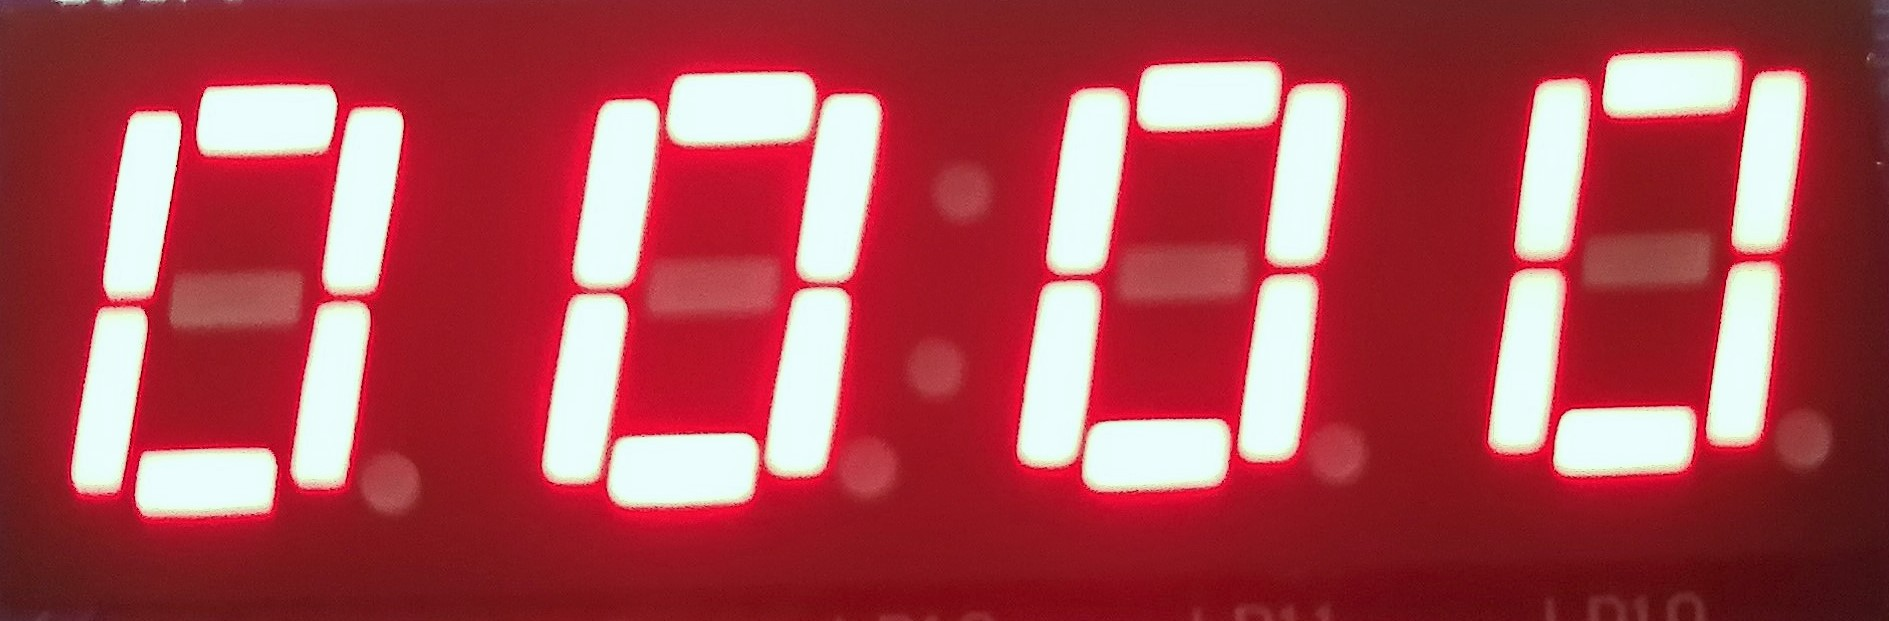
\includegraphics[width=0.3\linewidth]{fig/Implementation/0x00_01.jpg}\\
    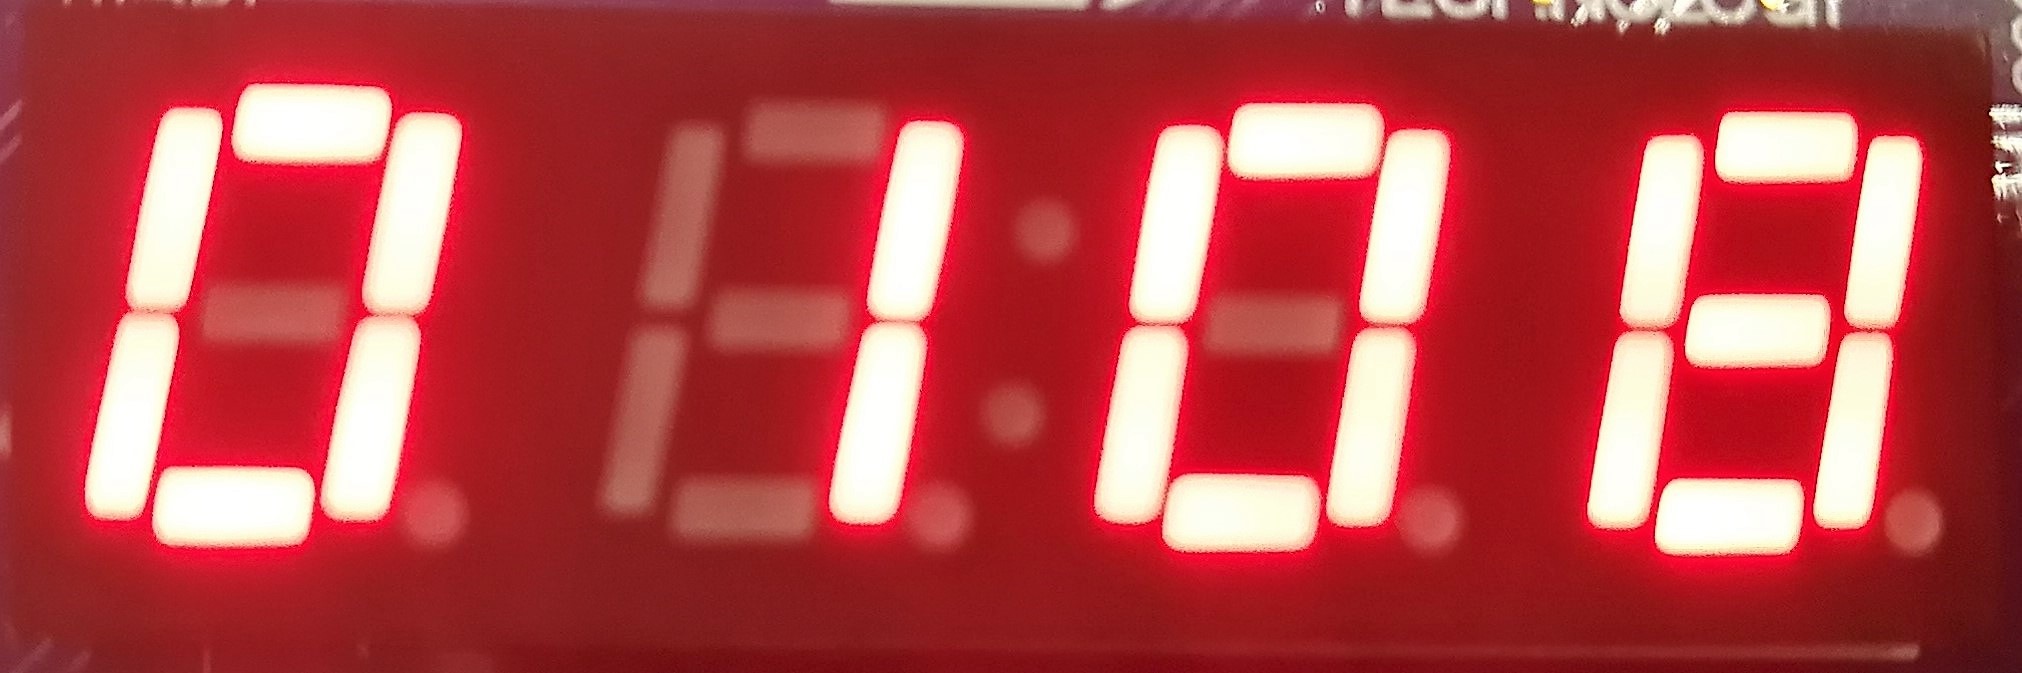
\includegraphics[width=0.3\linewidth]{fig/Implementation/0x00_10.jpg}&
    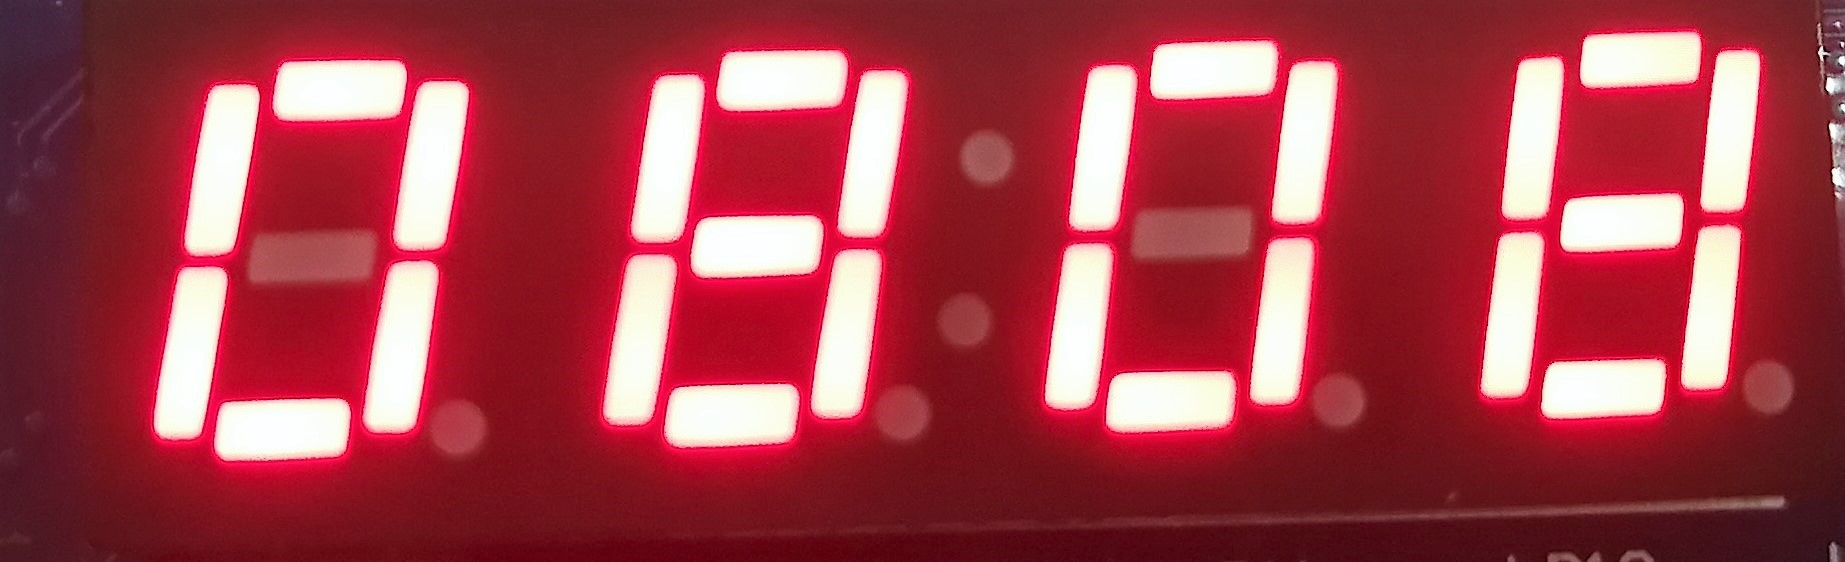
\includegraphics[width=0.3\linewidth]{fig/Implementation/0x00_11.jpg}
    \end{tabular}
    \caption{0x00结果}
    \end{figure}
    \item 0x14: \verb'sll $5, $5, 2'
    \begin{figure}[H]
    \centering
    \begin{tabular}{cc}
    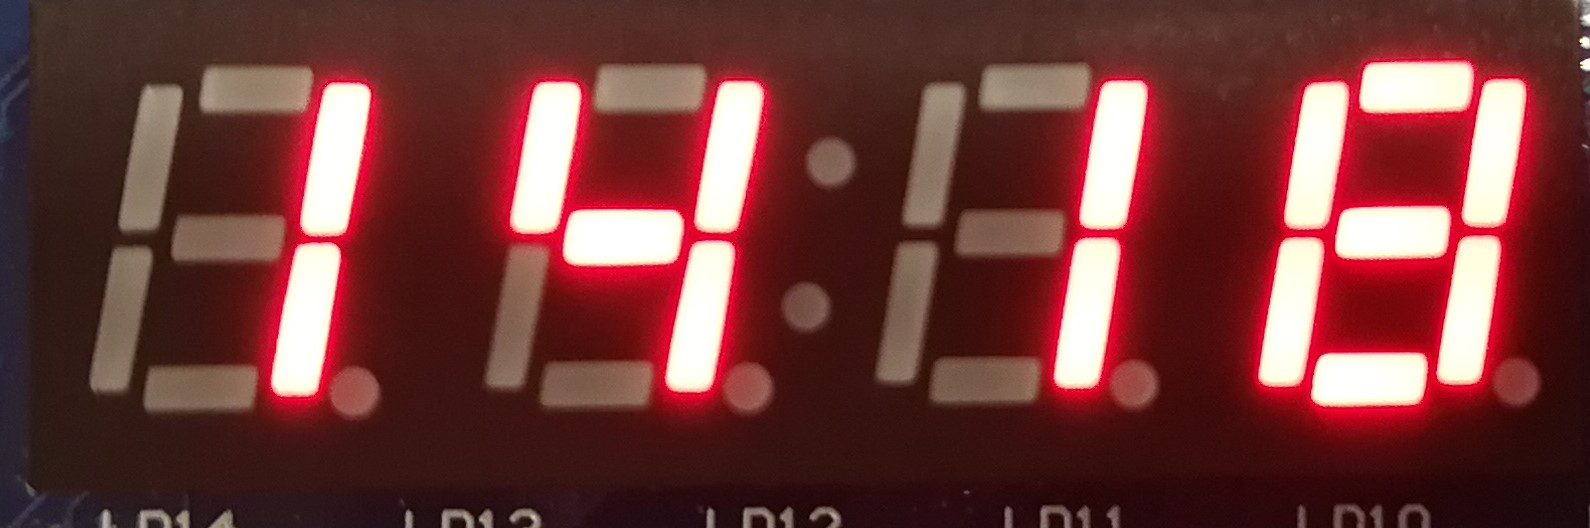
\includegraphics[width=0.3\linewidth]{fig/Implementation/0x14_00.jpg}&
    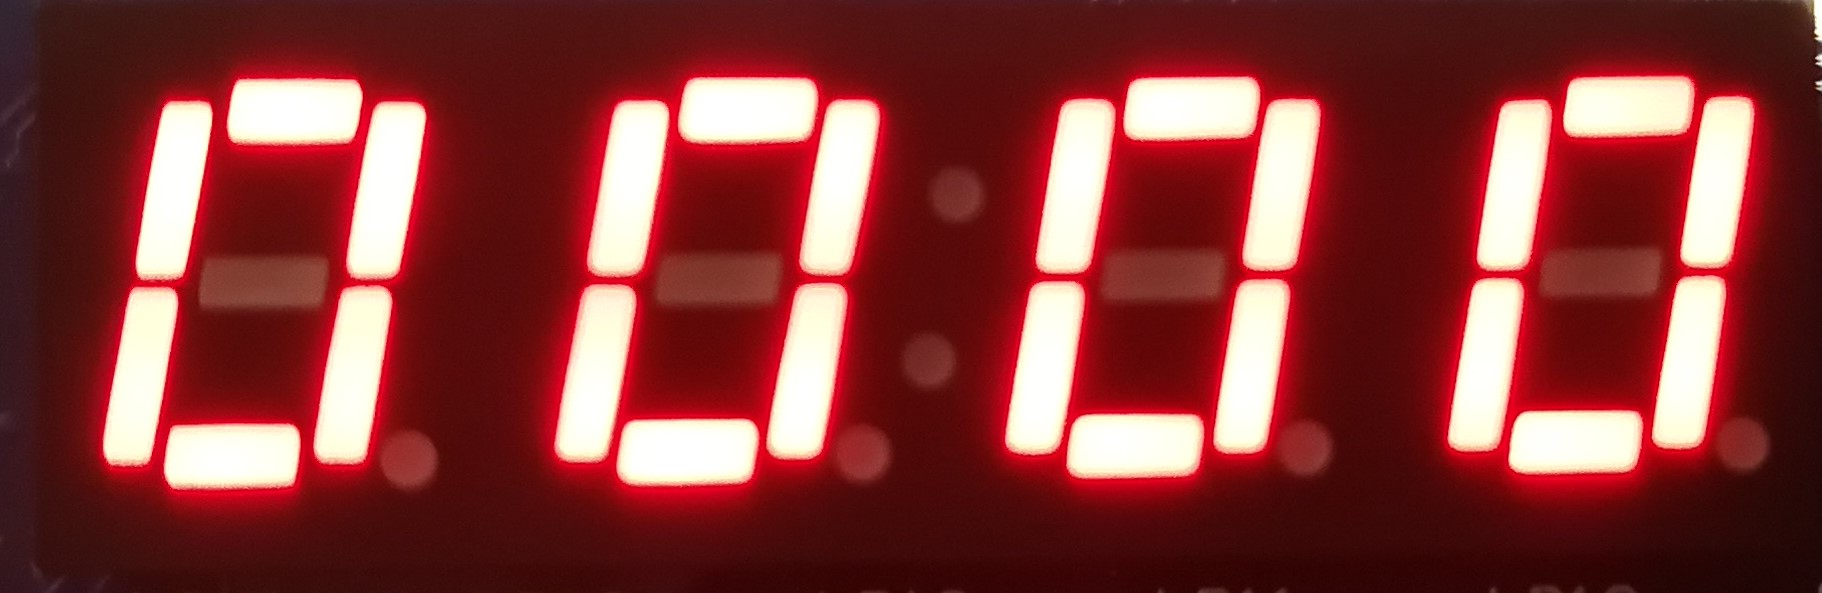
\includegraphics[width=0.3\linewidth]{fig/Implementation/0x14_01.jpg}\\
    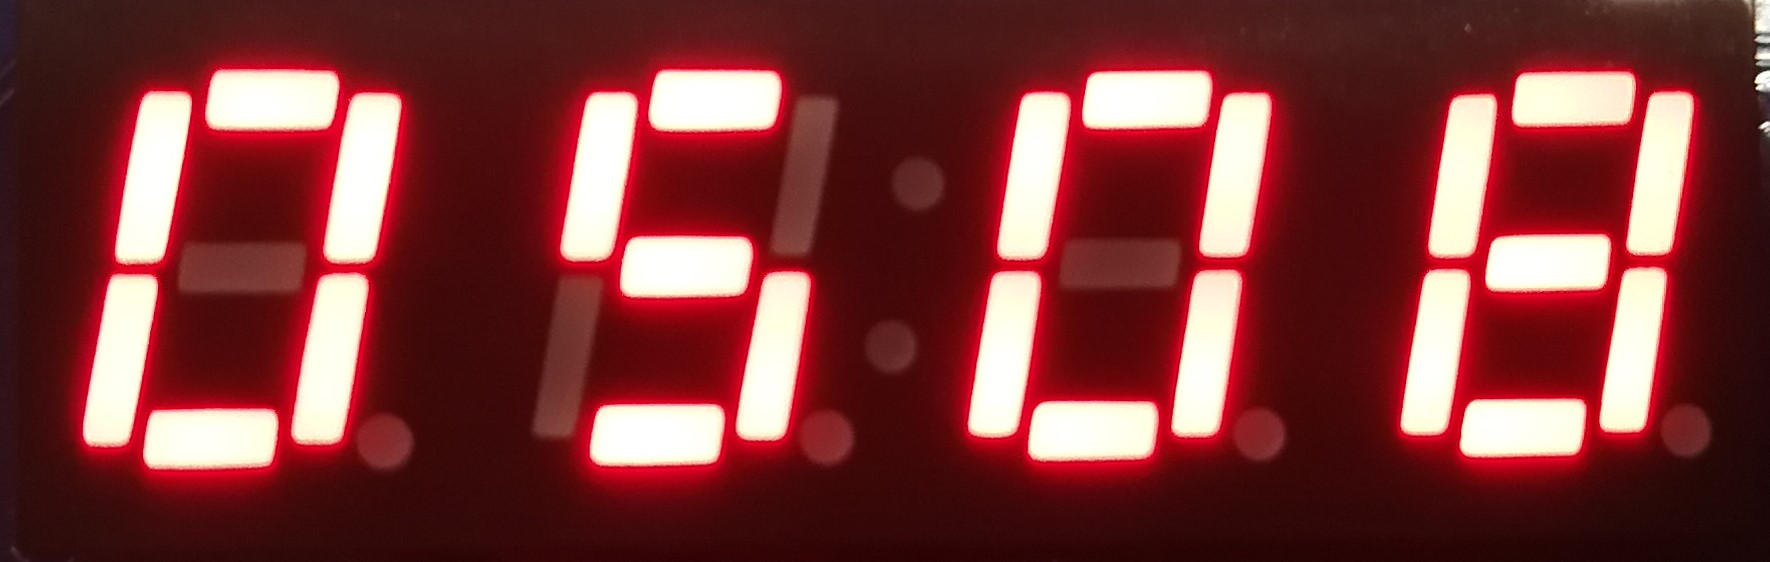
\includegraphics[width=0.3\linewidth]{fig/Implementation/0x14_10.jpg}&
    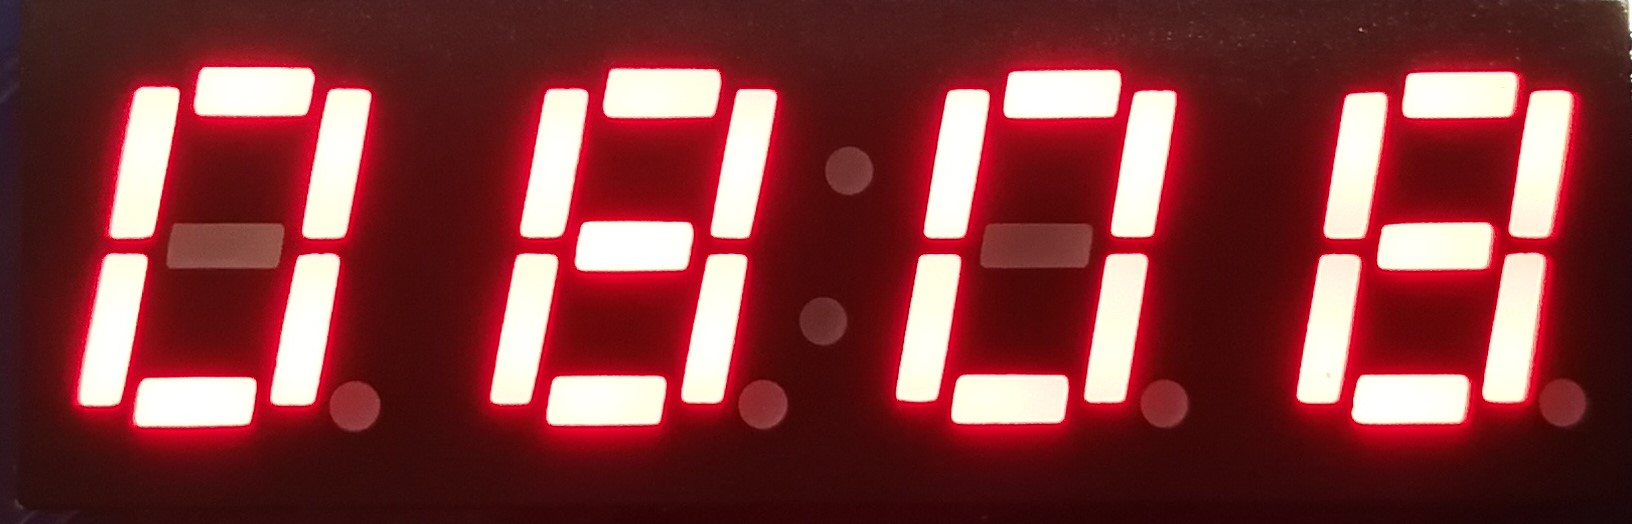
\includegraphics[width=0.3\linewidth]{fig/Implementation/0x14_11.jpg}
    \end{tabular}
    \caption{0x14结果}
    \end{figure}
    \item 0x18: \verb'beq $5, $1, -2'
    \begin{figure}[H]
    \centering
    \begin{tabular}{cc}
    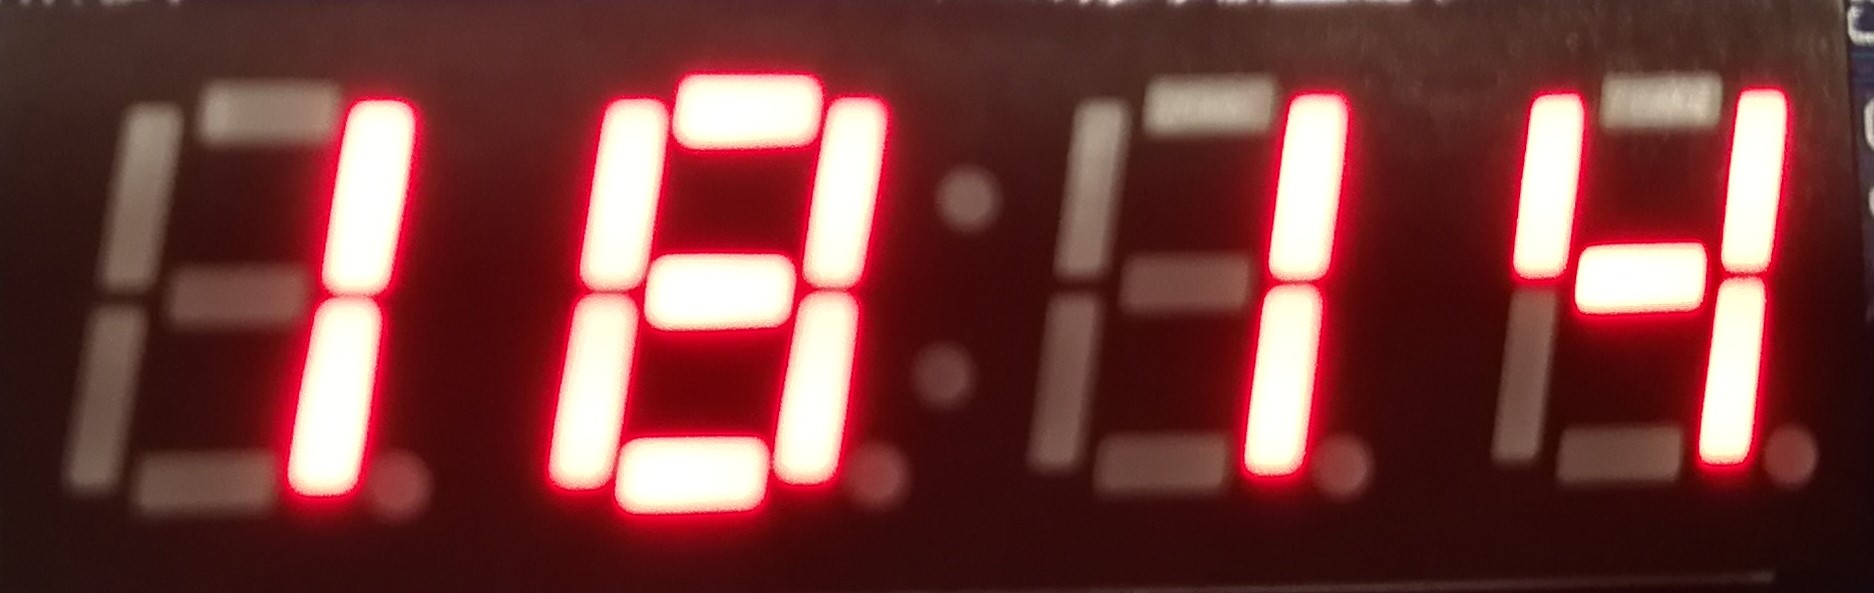
\includegraphics[width=0.3\linewidth]{fig/Implementation/0x18_00.jpg}&
    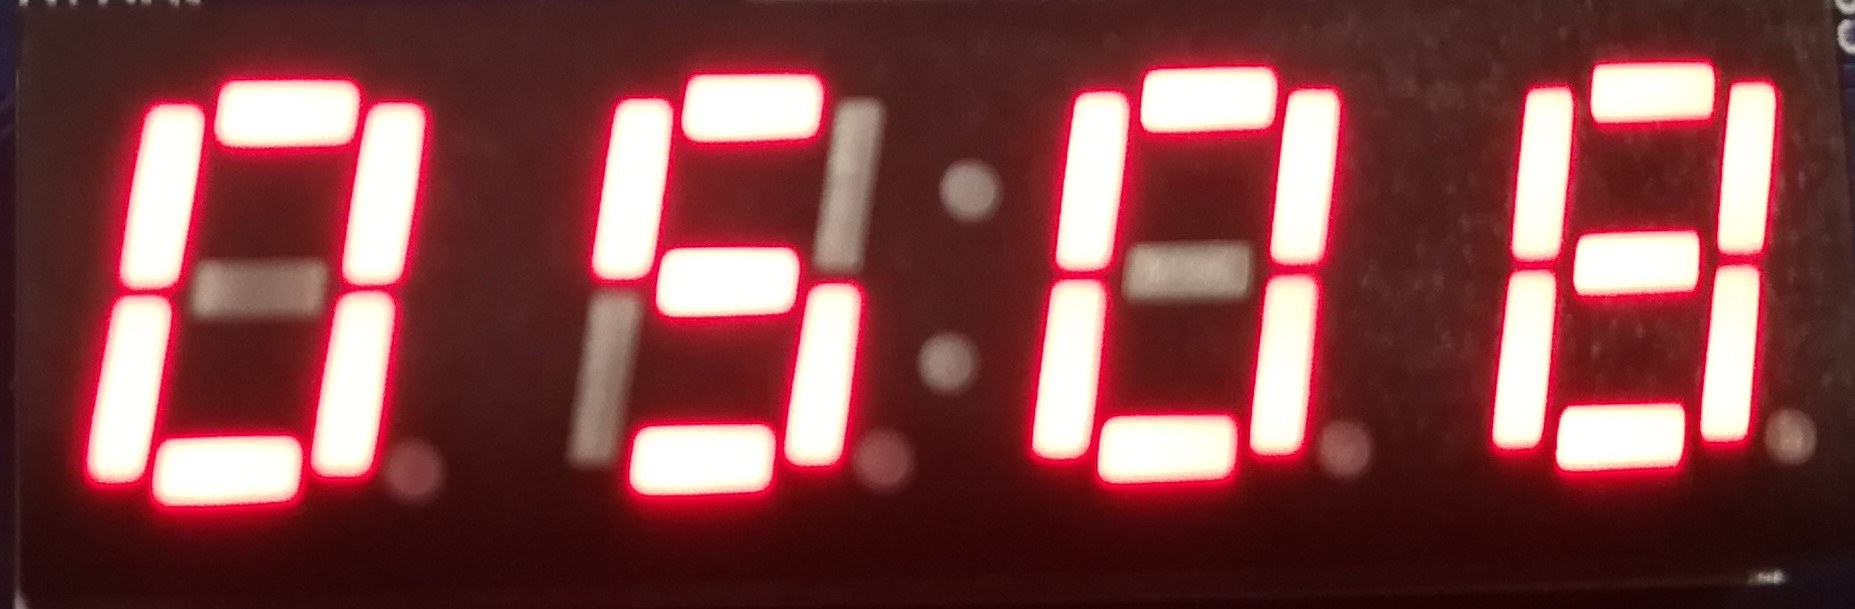
\includegraphics[width=0.3\linewidth]{fig/Implementation/0x18_01.jpg}\\
    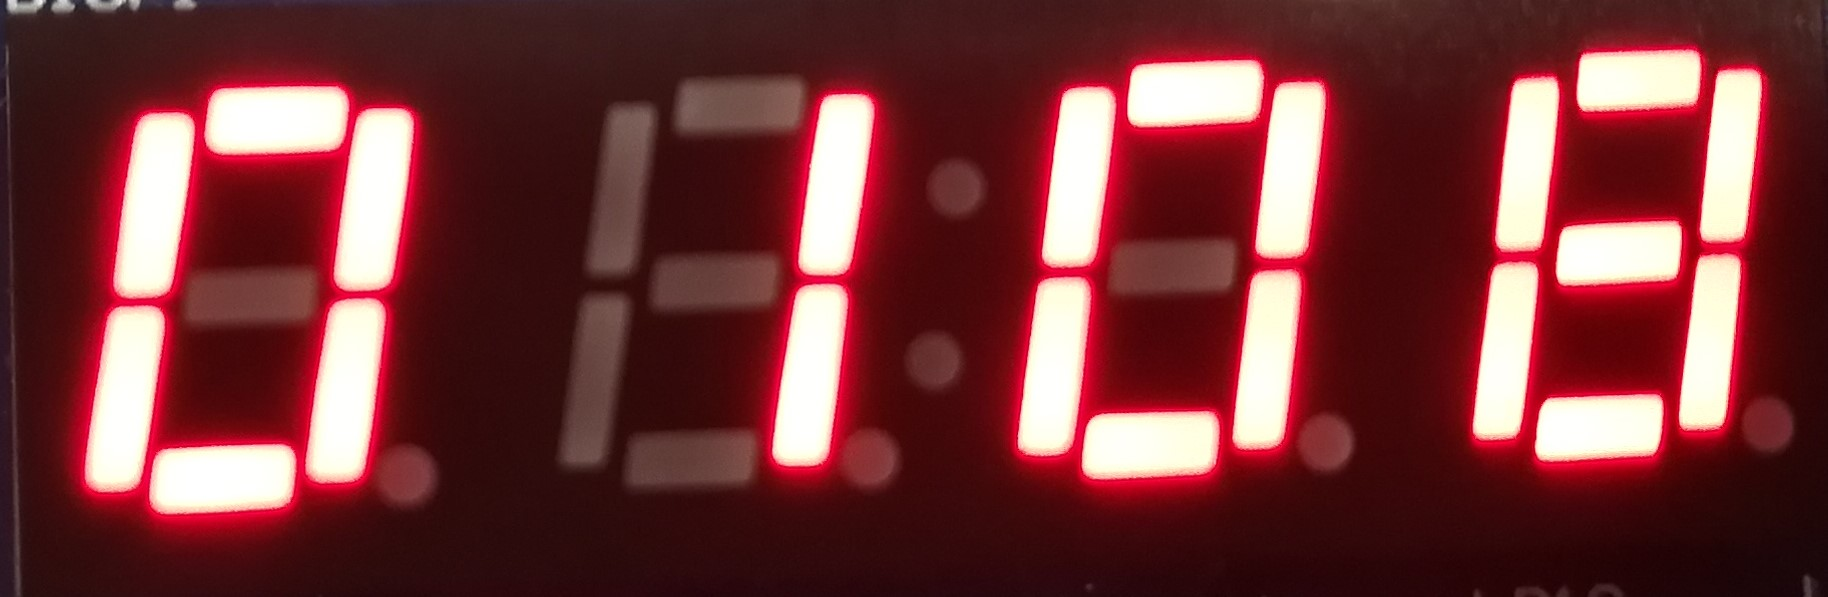
\includegraphics[width=0.3\linewidth]{fig/Implementation/0x18_10.jpg}&
    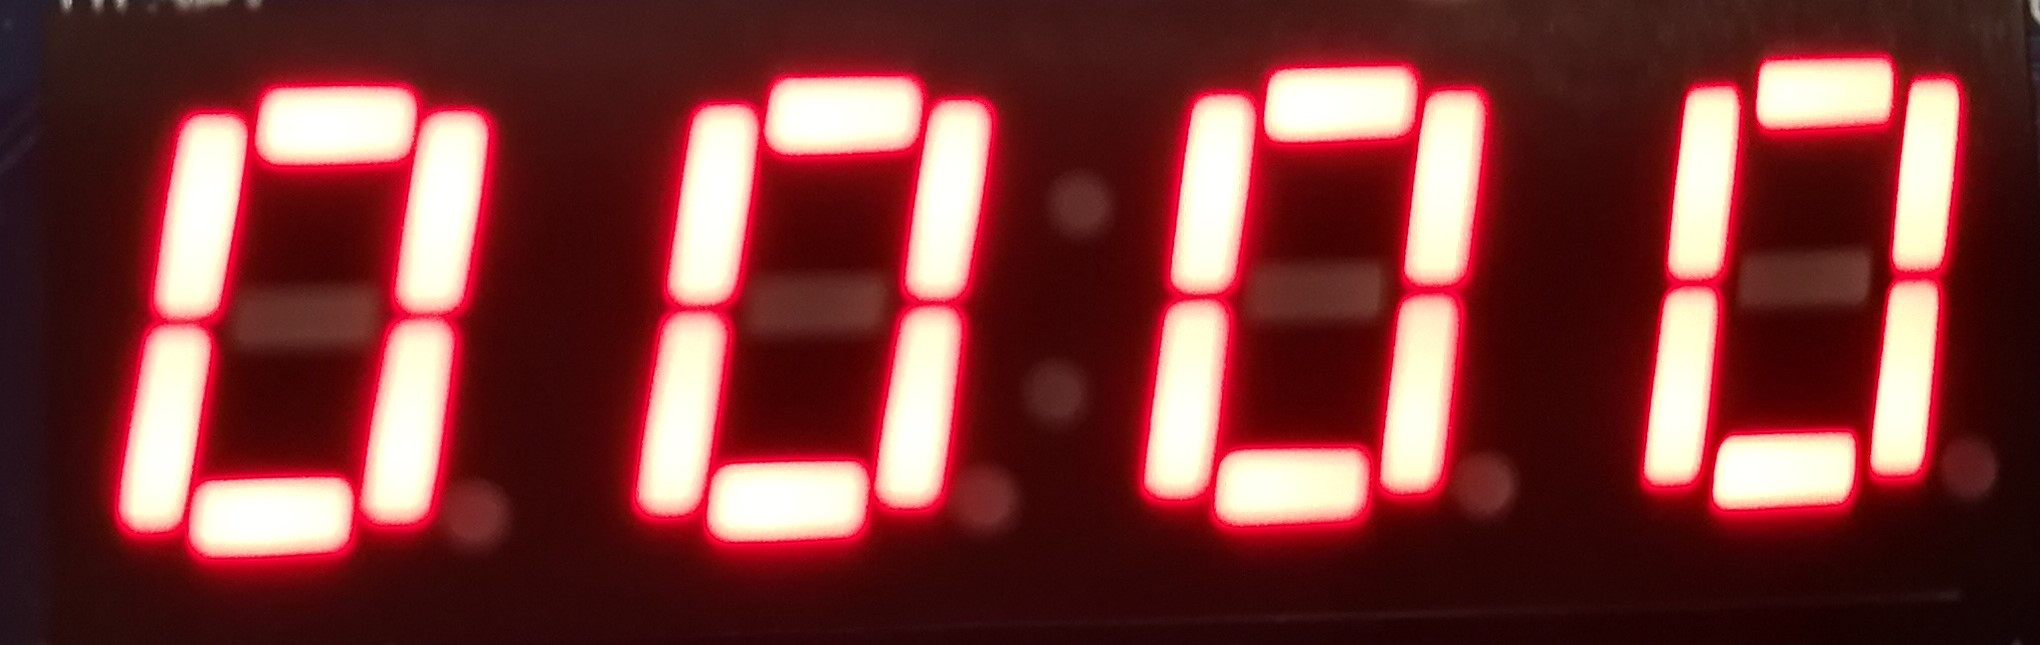
\includegraphics[width=0.3\linewidth]{fig/Implementation/0x18_11.jpg}
    \end{tabular}
    \caption{0x18结果}
    \end{figure}
    \item 0x1C: \verb'jal 0x0000050'
    \begin{figure}[H]
    \centering
    \begin{tabular}{cc}
    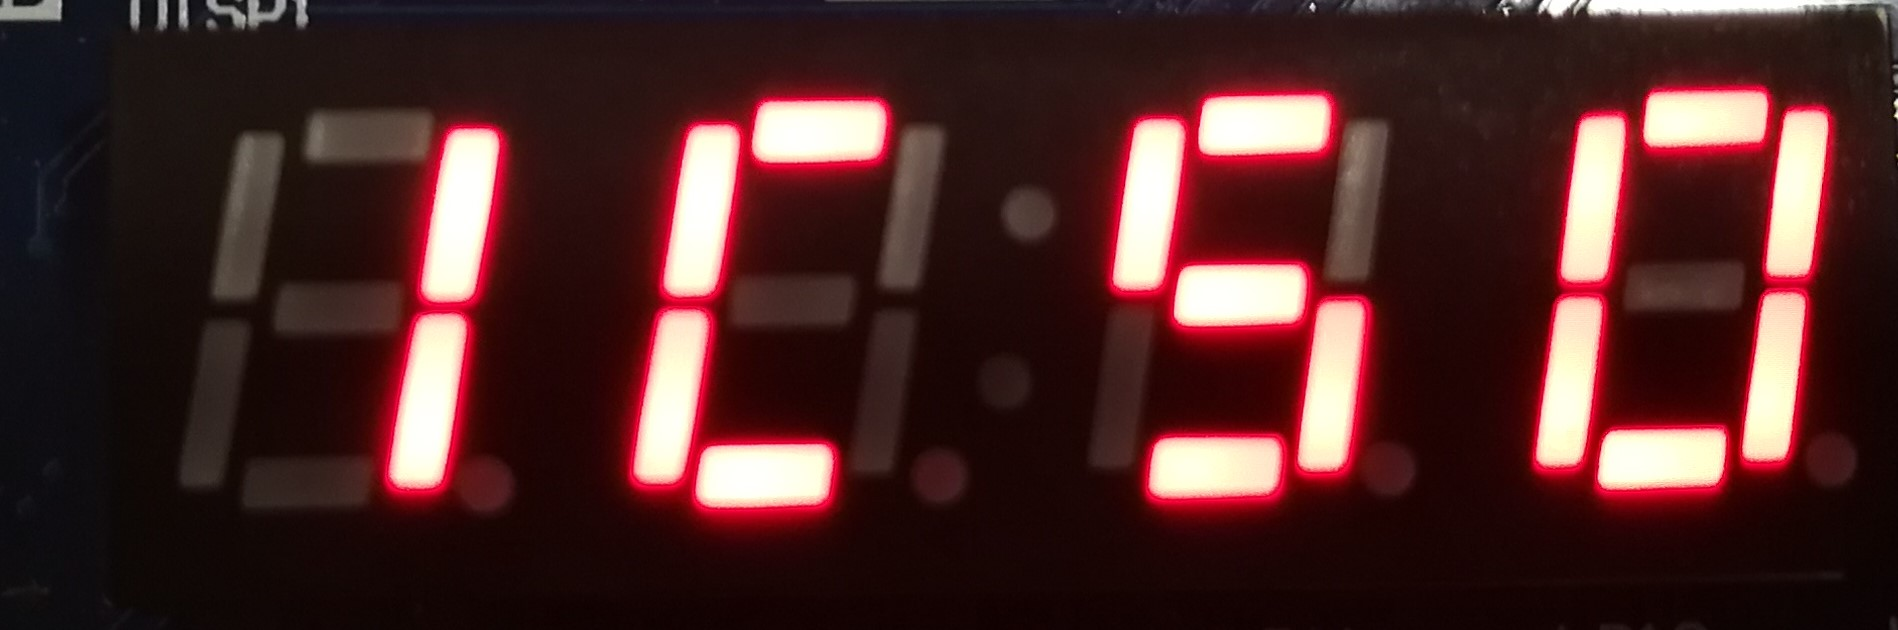
\includegraphics[width=0.3\linewidth]{fig/Implementation/0x1c_00.jpg}&
    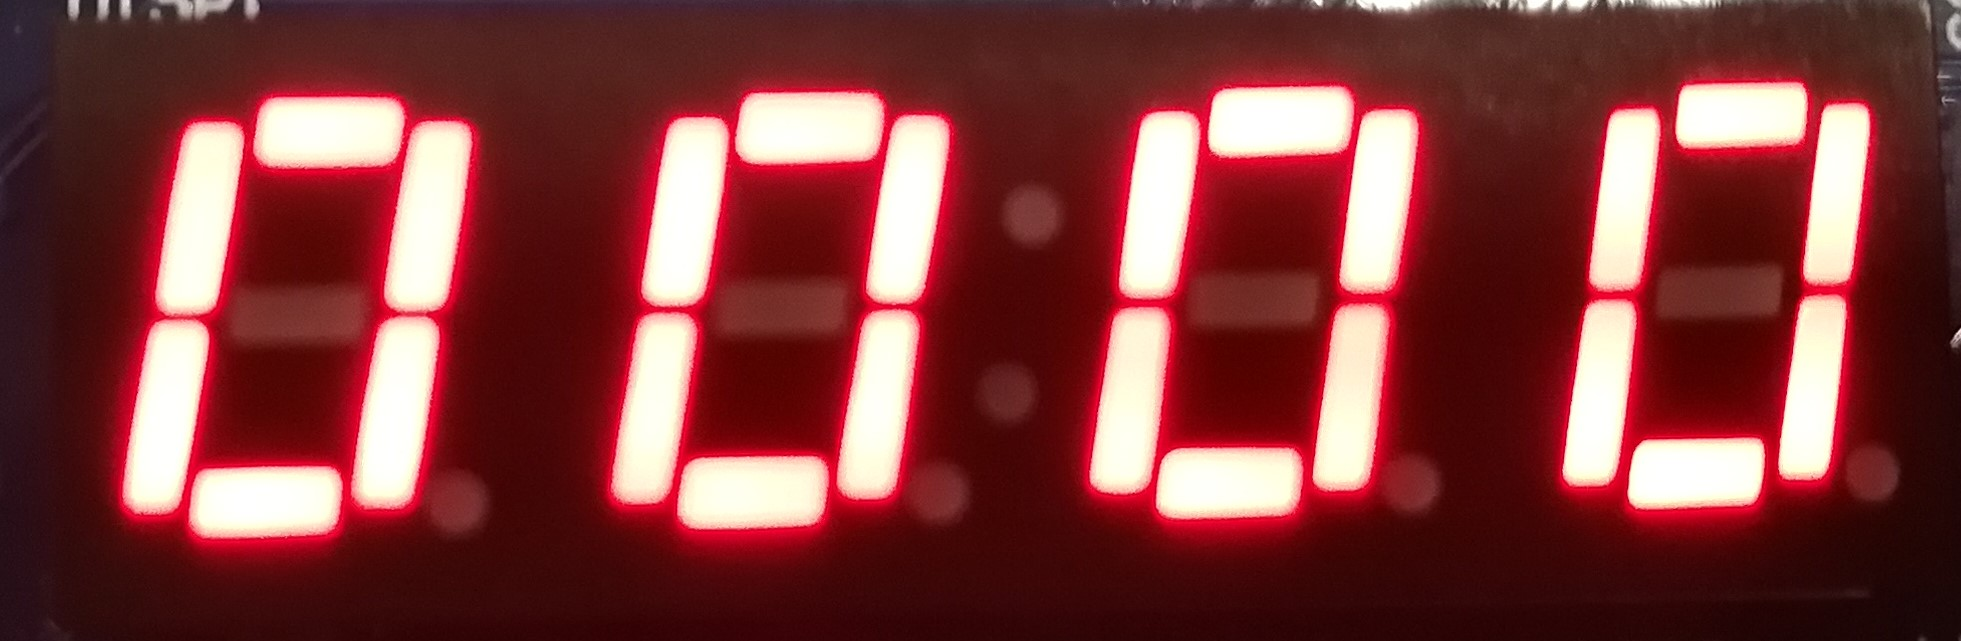
\includegraphics[width=0.3\linewidth]{fig/Implementation/0x1c_01.jpg}\\
    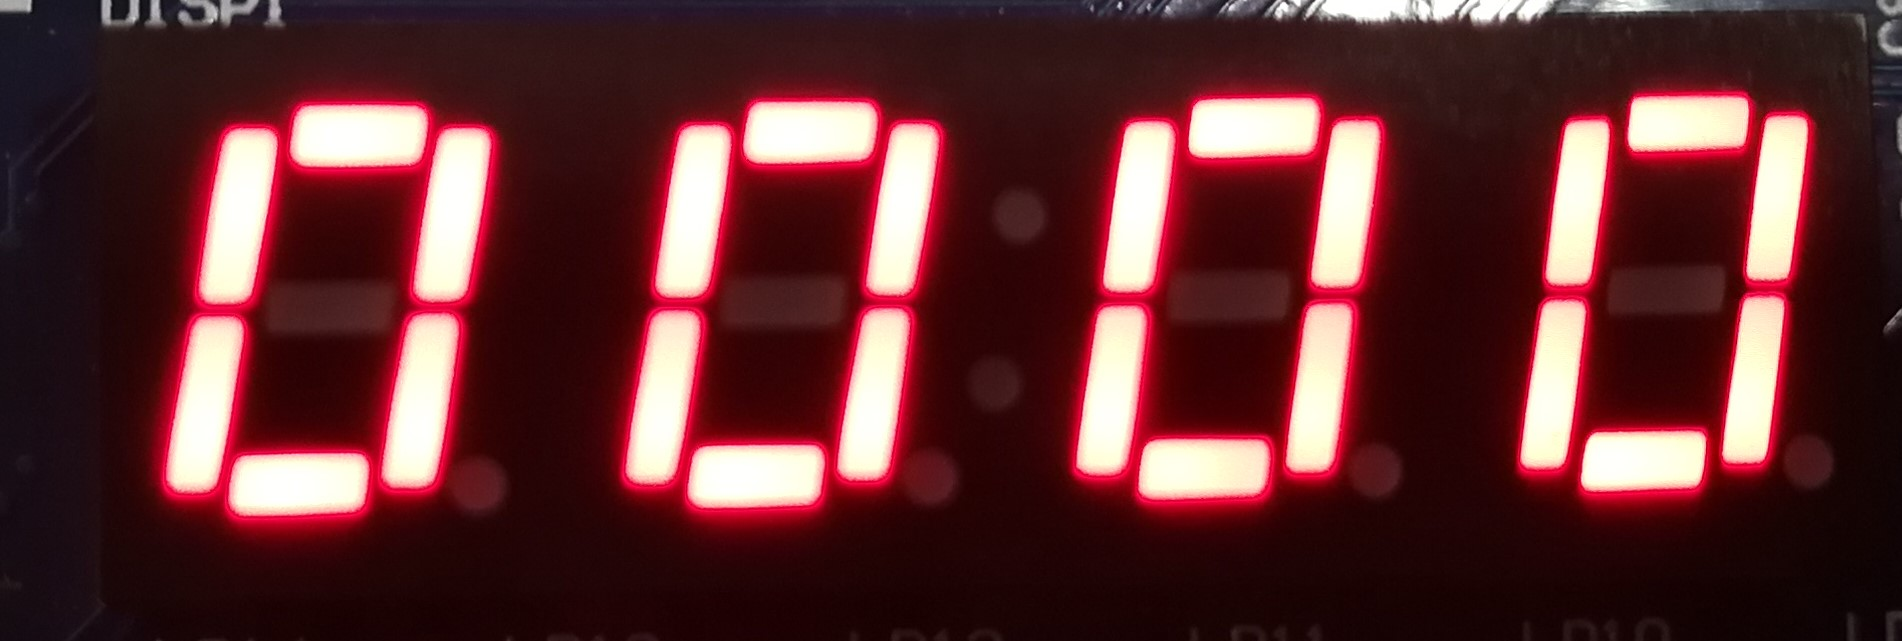
\includegraphics[width=0.3\linewidth]{fig/Implementation/0x1c_10.jpg}&
    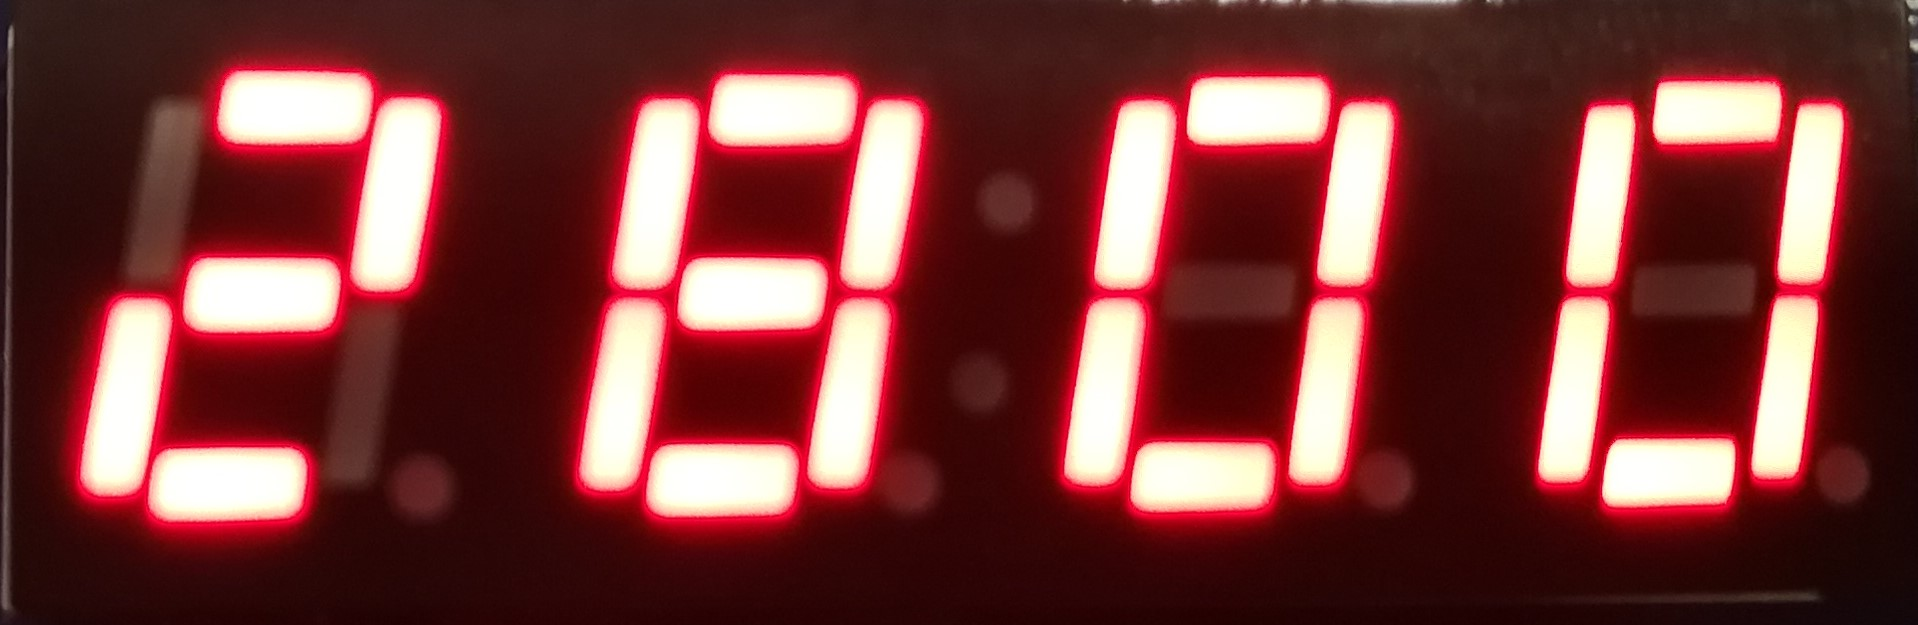
\includegraphics[width=0.3\linewidth]{fig/Implementation/0x1c_11.jpg}
    \end{tabular}
    \caption{0x1C结果}
    \end{figure}
    \item 0x54: \verb'lw $13, 4($1)'
    \begin{figure}[H]
    \centering
    \begin{tabular}{cc}
    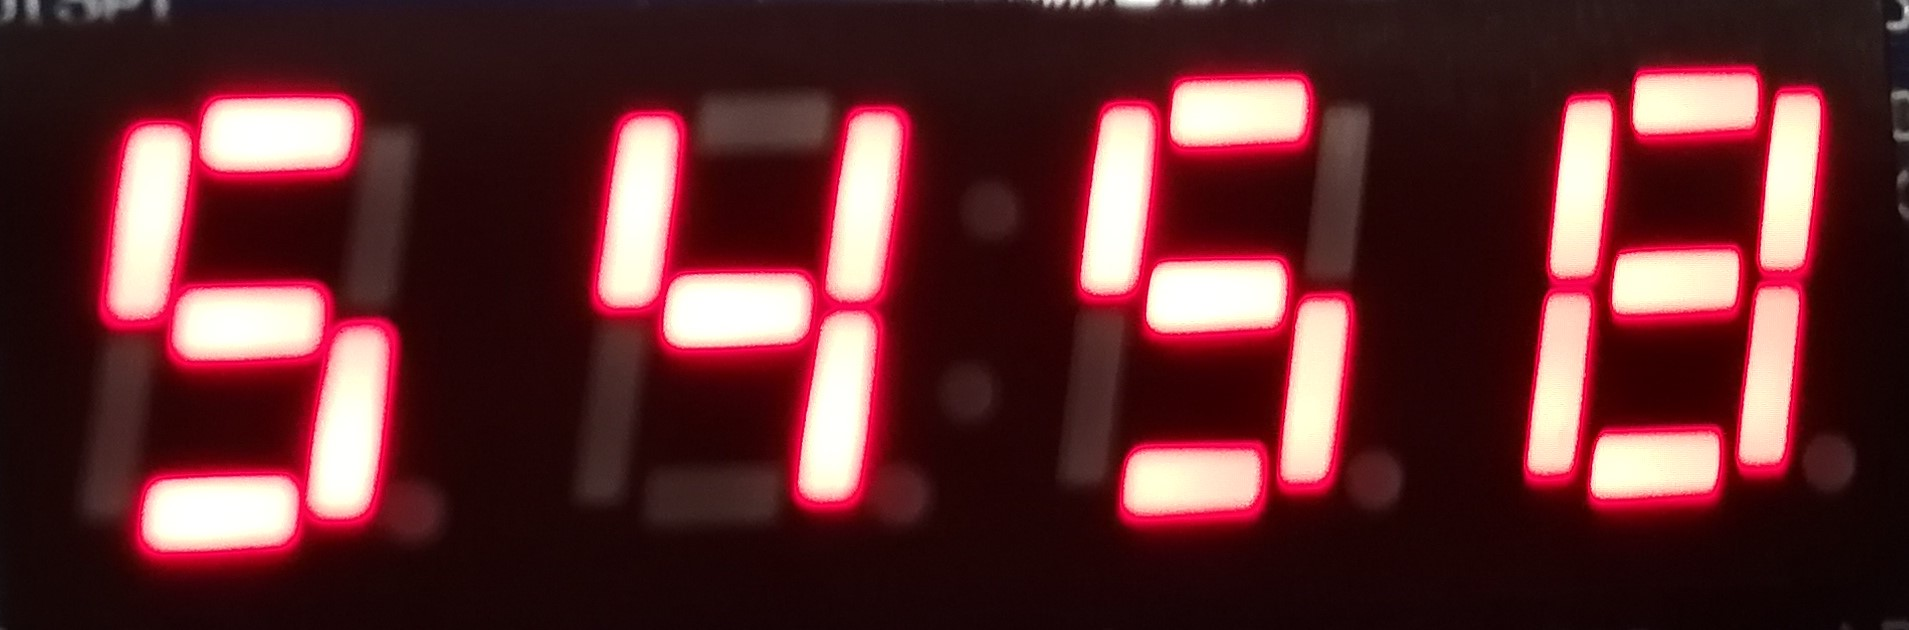
\includegraphics[width=0.3\linewidth]{fig/Implementation/0x54_00.jpg}&
    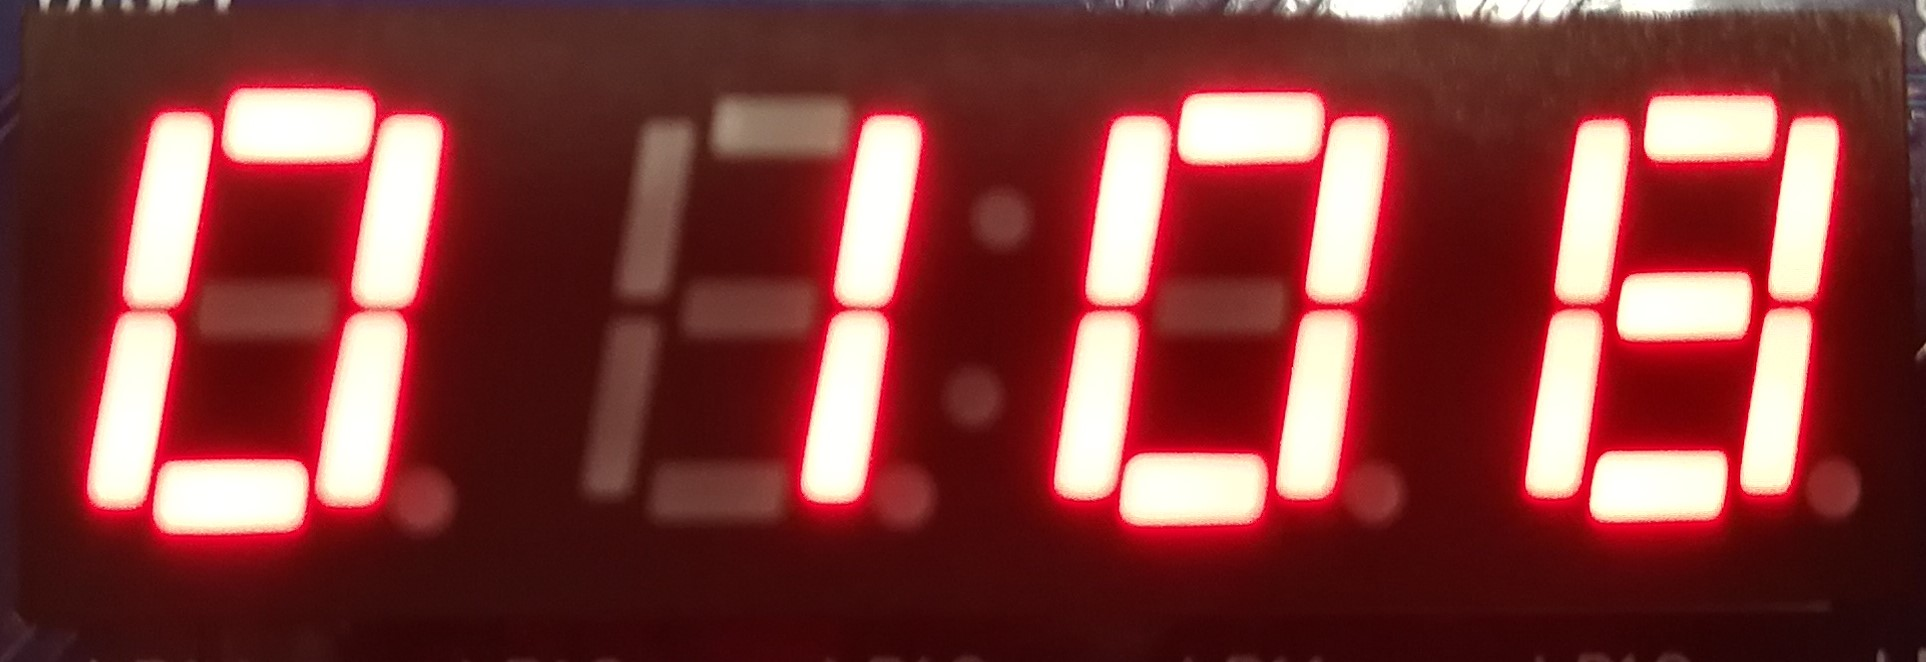
\includegraphics[width=0.3\linewidth]{fig/Implementation/0x54_01.jpg}\\
    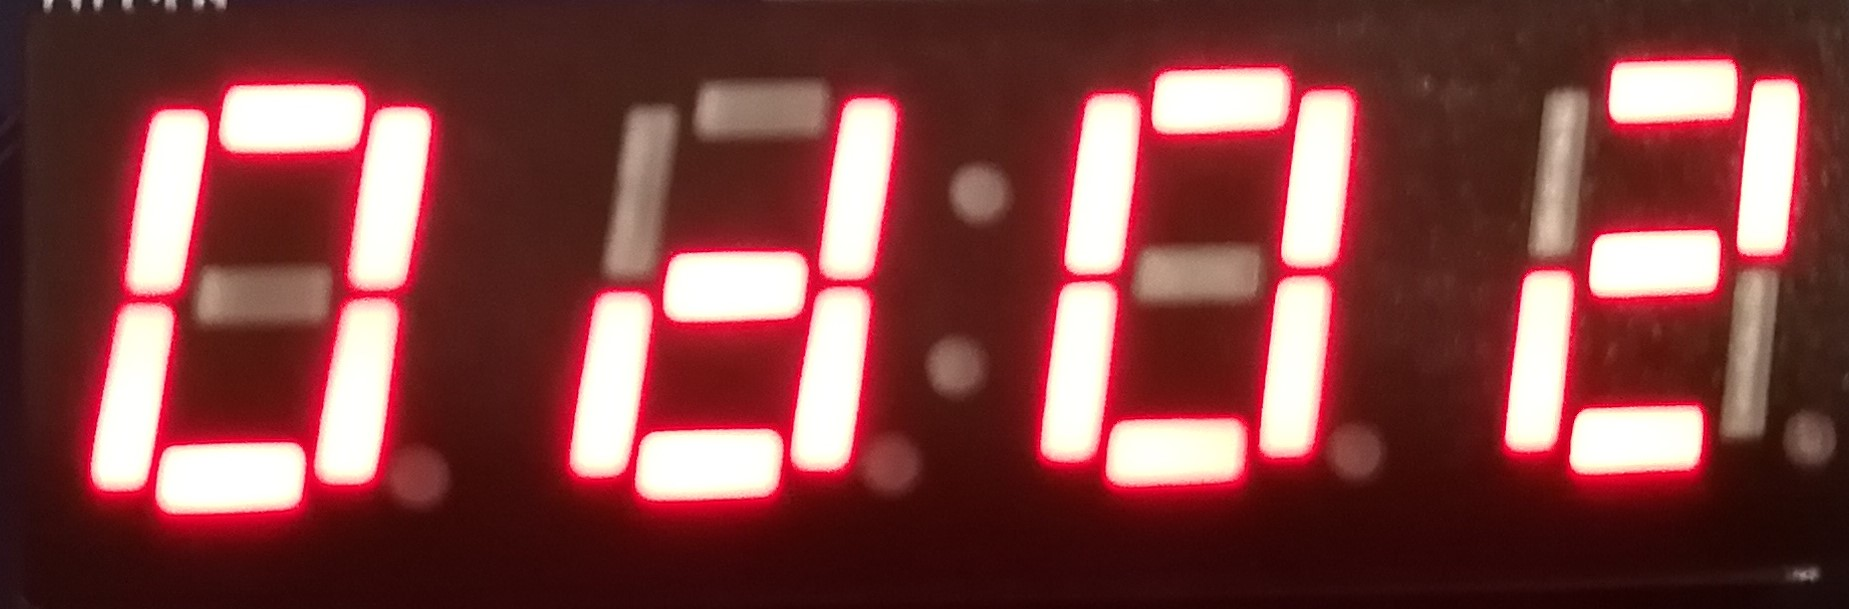
\includegraphics[width=0.3\linewidth]{fig/Implementation/0x54_10.jpg}&
    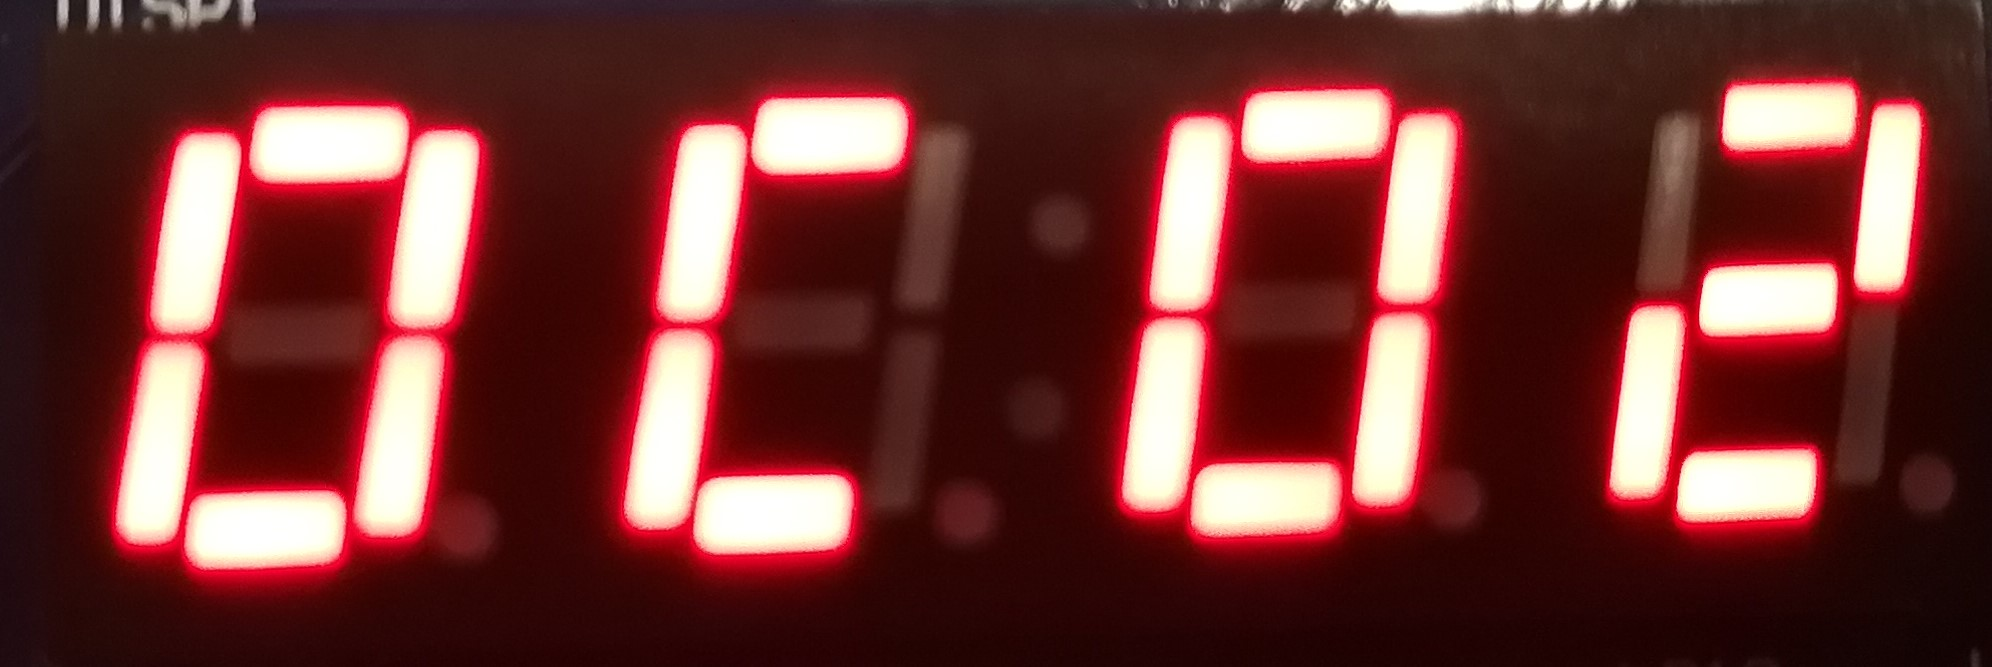
\includegraphics[width=0.3\linewidth]{fig/Implementation/0x54_11.jpg}
    \end{tabular}
    \caption{0x54结果}
    \end{figure}
    \item 0x58: \verb'jr $31'
    \begin{figure}[H]
    \centering
    \begin{tabular}{cc}
    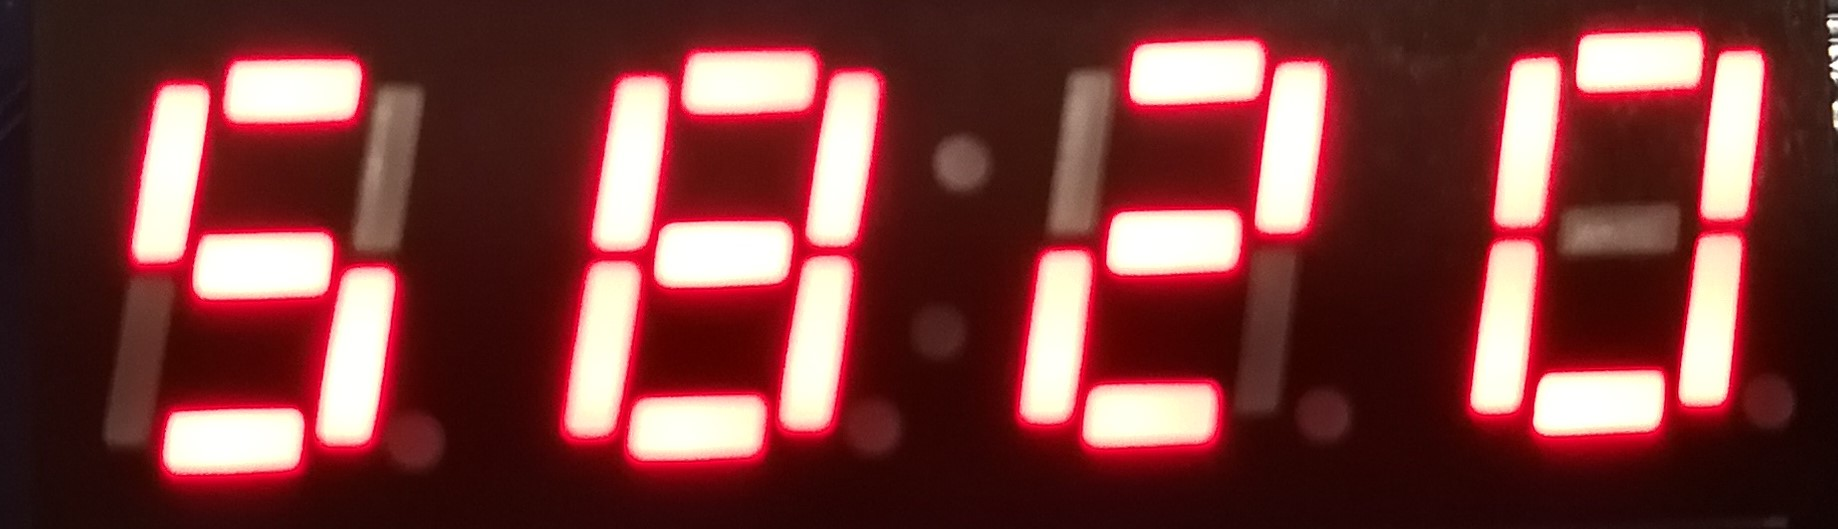
\includegraphics[width=0.3\linewidth]{fig/Implementation/0x58_00.jpg}&
    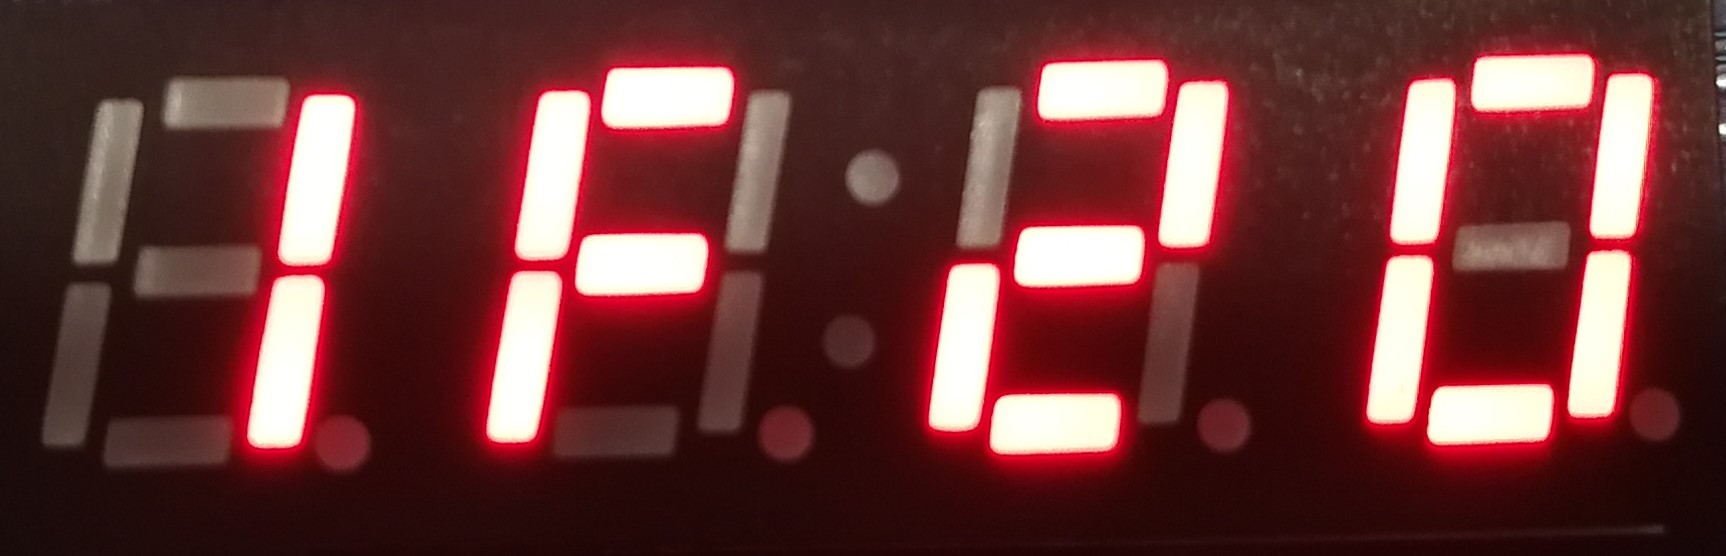
\includegraphics[width=0.3\linewidth]{fig/Implementation/0x58_01.jpg}\\
    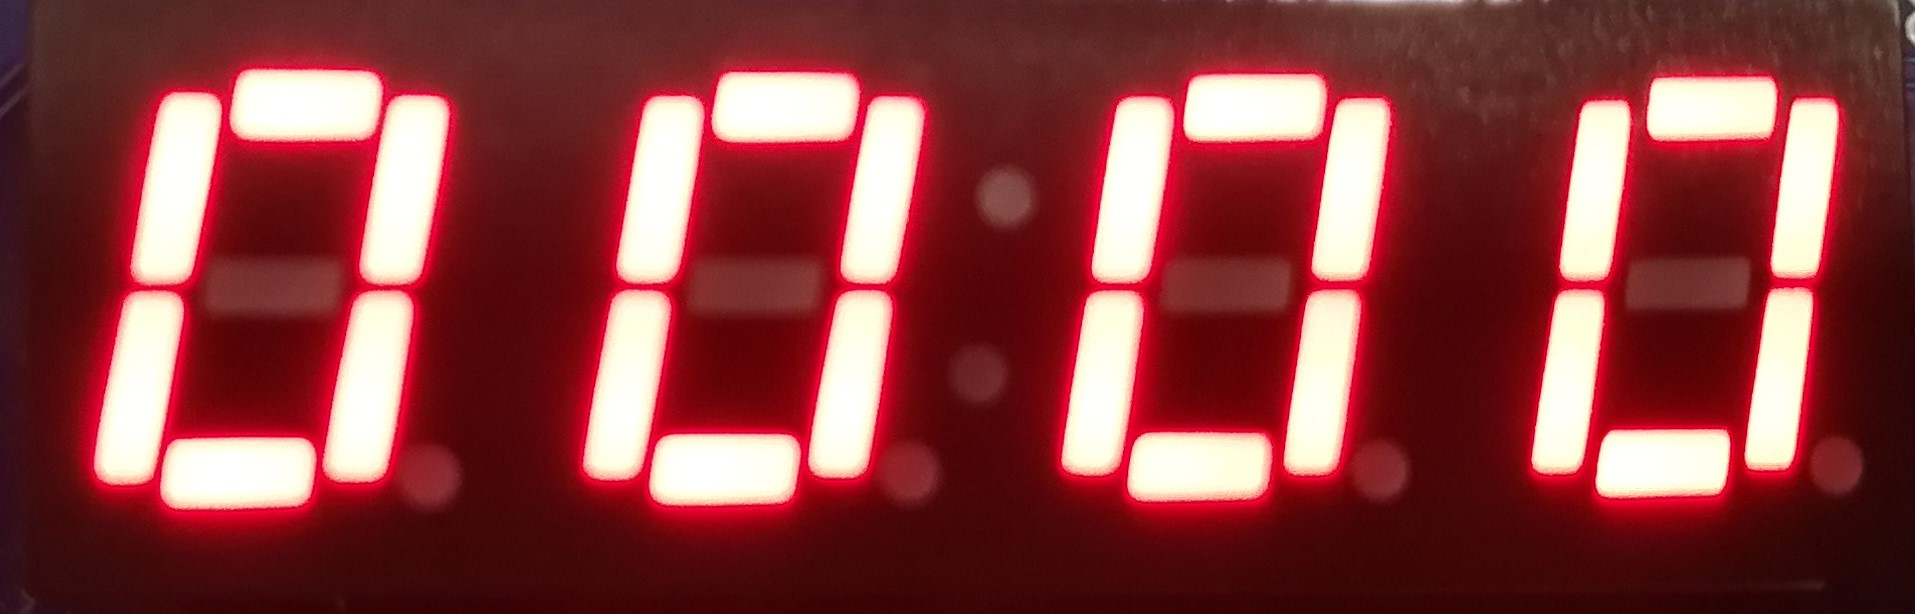
\includegraphics[width=0.3\linewidth]{fig/Implementation/0x58_10.jpg}&
    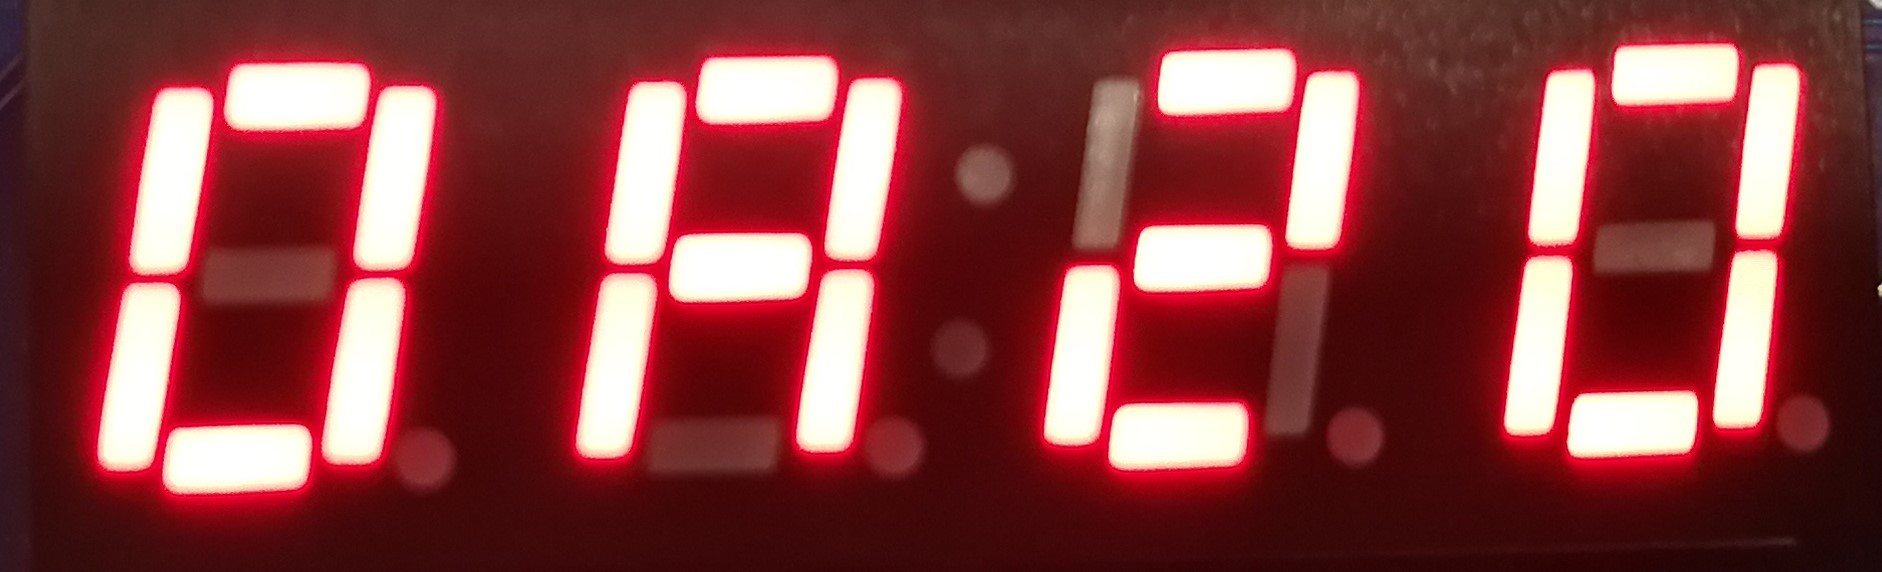
\includegraphics[width=0.3\linewidth]{fig/Implementation/0x58_11.jpg}
    \end{tabular}
    \caption{0x58结果}
    \end{figure}
\end{enumerate}